\documentclass[12pt]{article}
\usepackage{epsfig, epsf, graphicx, subfigure}
\usepackage{graphicx}
\usepackage{pstricks, pst-node, psfrag}
\usepackage{amssymb,amsmath}
\usepackage{verbatim,enumerate}
\usepackage{rotating, lscape}
\usepackage{multirow}
\usepackage{setspace}
\usepackage[square,sort,comma,numbers]{natbib}

\usepackage[hang, flushmargin]{footmisc}

\setlength{\oddsidemargin}{-0.125in}
\setlength{\topmargin}{-0.5in} \setlength{\textwidth}{6.5in}
\setlength{\textheight}{9in}

\setlength{\textheight}{9in} \setlength{\textwidth}{6.5in}
\setlength{\topmargin}{-40pt} \setlength{\oddsidemargin}{0pt}
\setlength{\evensidemargin}{0pt}
  
\setlength{\textheight}{9.4in} \setlength{\textwidth}{6.8in}
\setlength{\topmargin}{-71pt} \setlength{\oddsidemargin}{0pt}
\setlength{\evensidemargin}{-6pt} \tolerance=500
%\input psfig.tex
\setlength{\topmargin}{-56pt} \setlength{\oddsidemargin}{-6pt}
%%%%%%%%%%%%%%%%%%%%%%%%%%%%%%%%%%%%%%%%%%
\def\wt{\widetilde}
\def\diag{\hbox{diag}}
\def\wh{\widehat}
\def\AIC{\hbox{AIC}}
\def\BIC{\hbox{BIC}}
\def\sm{\footnotesize}
%- Makes the section title start with Appendix in the appendix environment
\newcommand{\Appendix}
{%\appendix
\def\thesection{Appendix~\Alph{section}}
%\def\thesubsection{\Alph{section}.\arabic{subsection}}
\def\thesubsection{A.\arabic{subsection}}
}
\def\diag{\hbox{diag}}
\def\log{\hbox{log}}
\def\bias{\hbox{bias}}
\def\Siuu{\boldSigma_{i,uu}}
\def\ANNALS{{\it Annals of Statistics}}
\def\BIOK{{\it Biometrika}}
\def\whT{\widehat{\Theta}}
\def\STATMED{{\it Statistics in Medicine}}
\def\STATSCI{{\it Statistical Science}}
\def\JSPI{{\it Journal of Statistical Planning \&amp; Inference}}
\def\JRSSB{{\it Journal of the Royal Statistical Society, Series B}}
\def\BMCS{{\it Biometrics}}
\def\COMMS{{\it Communications in Statistics, Theory \& Methods}}
\def\JQT{{\it Journal of Quality Technology}}
\def\STIM{{\it Statistics in Medicine}}
\def\TECH{{\it Technometrics}}
\def\AJE{{\it American Journal of Epidemiology}}
\def\JASA{{\it Journal of the American Statistical Association}}
\def\CDA{{\it Computational Statistics \& Data Analysis}}
\def\JCGS{{\it Journal of Computational and Graphical Statistics}}
\def\JCB{{\it Journal of Computational Biology}}
\def\BIOINF{{\it Bioinformatics}}
\def\JAMA{{\it Journal of the American Medical Association}}
\def\JNUTR{{\it Journal of Nutrition}}
\def\JCGS{{\it Journal of Computational and Graphical Statistics}}
\def\LETTERS{{\it Letters in Probability and Statistics}}
\def\JABES{{\it Journal of Agricultural and
                      Environmental Statistics}}
\def\JASA{{\it Journal of the American Statistical Association}}
\def\ANNALS{{\it Annals of Statistics}}
\def\JSPI{{\it Journal of Statistical Planning \& Inference}}
\def\TECH{{\it Technometrics}}
\def\BIOK{{\it Bio\-me\-tri\-ka}}
\def\JRSSB{{\it Journal of the Royal Statistical Society, Series B}}
\def\BMCS{{\it Biometrics}}
\def\COMMS{{\it Communications in Statistics, Series A}}
\def\JQT{{\it Journal of Quality Technology}}
\def\SCAN{{\it Scandinavian Journal of Statistics}}
\def\AJE{{\it American Journal of Epidemiology}}
\def\STIM{{\it Statistics in Medicine}}
\def\ANNALS{{\it Annals of Statistics}}
\def\whT{\widehat{\Theta}}
\def\STATMED{{\it Statistics in Medicine}}
\def\STATSCI{{\it Statistical Science}}
\def\JSPI{{\it Journal of Statistical Planning \& Inference}}
\def\JRSSB{{\it Journal of the Royal Statistical Society, Series B}}
\def\BMCS{{\it Biometrics}}
\def\COMMS{{\it Communications in Statistics, Theory \& Methods}}
\def\JQT{{\it Journal of Quality Technology}}
\def\STIM{{\it Statistics in Medicine}}
\def\TECH{{\it Technometrics}}
\def\AJE{{\it American Journal of Epidemiology}}
\def\JASA{{\it Journal of the American Statistical Association}}
\def\CDA{{\it Computational Statistics \& Data Analysis}}
\def\dfrac#1#2{{\displaystyle{#1\over#2}}}
\def\VS{{\vskip 3mm\noindent}}
\def\boxit#1{\vbox{\hrule\hbox{\vrule\kern6pt
          \vbox{\kern6pt#1\kern6pt}\kern6pt\vrule}\hrule}}
\def\refhg{\hangindent=20pt\hangafter=1}
\def\refmark{\par\vskip 2mm\noindent\refhg}
\def\naive{\hbox{naive}}
\def\itemitem{\par\indent \hangindent2\pahttprindent \textindent}
\def\var{\hbox{var}}
\def\cov{\hbox{cov}}
\def\corr{\hbox{corr}}
\def\trace{\hbox{trace}}
\def\refhg{\hangindent=20pt\hangafter=1}
\def\refmark{\par\vskip 2mm\noindent\refhg}
\def\Normal{\hbox{Normal}}
\def\povr{\buildrel p\over\longrightarrow}
\def\ccdot{{\bullet}}
\def\bse{\begin{eqnarray*}}
\def\ese{\end{eqnarray*}}
\def\be{\begin{eqnarray}}
\def\ee{\end{eqnarray}}
\def\bq{\begin{equation}}
\def\eq{\end{equation}}
\def\bse{\begin{eqnarray*}}
\def\ese{\end{eqnarray*}}
\def\pr{\hbox{pr}}
\def\wh{\widehat}
\def\trans{^{\rm T}}
\def\myalpha{{\cal A}}
\def\th{^{th}}
%%%%%%%%%%%%%%%%%%%%%%%%%%%%%%%%%%%%%%%%%%%%%%%%%%%%%%%%%%%%%%%%%%%%%%%%%%%%%
% Marc Definitions
%%%%%%%%%%%%%%%%%%%%%%%%%%%%%%%%%%%%%%%%%%%%%%%%%%%%%%%%%%%%%%%%%%%%%%%%%%%%%
\renewcommand{\baselinestretch}{1.2} % Change this 1.5 or whatever
\newcommand{\qed}{\hfill\hfill\vbox{\hrule\hbox{\vrule\squarebox
   {.667em}\vrule}\hrule}\smallskip}
\newtheorem{Th}{Theorem}
\newtheorem{Proof}{Proof}
\newtheorem{Mth}{Main Theorem}
\newtheorem{Def}{Definition}
\newtheorem{Rem}{Remark}
\newtheorem{Qes}{Question}
\newtheorem{proposition}{Proposition}
\newtheorem{Lem}{Lemma}
\newtheorem{Cor}{Corollary}
\newtheorem{Exa}{Example}
\newtheorem{Eq}{Equation}
%\renewcommand{\baselinestretch}{1.5}
\def\btheta{{\boldsymbol \theta}}
\def\balpha{{\boldsymbol \alpha}}
\def\bmu{{\boldsymbol \mu}}
\def\bpi{{\boldsymbol \pi}}
\def\x{{\bf x}}
\def\a{{\bf a}}
\def\mA{\mathcal{A}}
\def\mB{\mathcal{B}}
\def\mC{\mathcal{C}}
\def\mH{\mathcal{H}}
\def\mR{\mathcal{R}}
\def\mD{\mathcal{D}}

\newtheorem{lemm}{Lemma}[section]
\newtheorem{thm}{Theorem}[section]
\newtheorem{cor}{Corollary}[thm]
\newtheorem{defi}{Definition}
\newtheorem{prop}{Proposition}
\newtheorem{example}{Example}

\def\bX{{\bf X}}
\def\bY{{\bf Y}}
\def\bZ{{\bf Z}}
\def\bU{{\bf U}}
\def\bT{{\bf T}}
\def\bV{{\bf V}}
\def\bx{{\bf x}}
\def\by{{\bf y}}
\def\bz{{\bf z}}
\def\bu{{\bf u}}
\def\bv{{\bf v}}
\def\bs{{\bf s}}
\def\ba{{\bf a}}
\def\bb{{\bf b}}
\def\bmu{{\boldsymbol \mu}}
\def\bbeta{{\boldsymbol \beta}}
\def\balpha{{\boldsymbol \alpha}}
\def\bxi{{\boldsymbol \xi}}
\def\bdelta{{\boldsymbol \delta}}
\def\blambda{{\boldsymbol \lambda}}
\def\btheta{{\boldsymbol \theta}}
\def\beeta{{\boldsymbol \eta}}
\def\bupsilon{{\boldsymbol \upsilon}}
\def\R{\mathbb R}


%\newcommand{\pr}{\mbox{Pr}}
%\newcommand{\var}{\mbox{var}}
%\newcommand{\cov}{\mbox{cov}}
%\newcommand{\logit}{\mbox{logit }}
\newcommand{\cp}{\stackrel{\mathcal{P}}{\rightarrow}}
\newcommand{\cl}{\stackrel{\mathcal{D}}{\rightarrow}}
\newcommand{\mystrut}{\vphantom{\int_0^1}}
\newcommand{\p}{\stackrel{p}{\rightarrow}}
\renewcommand{\d}{\stackrel{d}{\rightarrow}}
\newcommand{\condind}{\perp\hspace{-1em}\perp}
\newcommand{\sumi}{\ensuremath{\sum_{i=1}^{n}}}
\newcommand{\sumj}{\ensuremath{\sum_{j=1}^{n}}}
\newcommand{\eff}{\mbox{\scriptsize eff}}
\def\my{\mathcal Y}




\def\nh{\noindent\hangindent=1.5truecm\hangafter=1}
\def\cl{\centerline}
\def\ms{\medskip}
\def\ni{\noindent}
\def\ve{\vfill\eject}

\def\A{{\rm A}}
\def\ab{\allowbreak}
\def\bigmi{\,\big|\,}
\def\cI{{\cal I}}
\def\cT{{\cal T}}
\def\dt{{\dot t}}
\def\da{{\dot a}}
\def\dar{\downarrow}
\def\ddt{{\ddot t}}
\def\de{\delta}
\def\De{\Delta}
\def\ep{\epsilon}
\def\gz{g_0}
\def\ha{{\hat a}}
\def\half{^{1/2}}
\def\hg{{\hat g}}
\def\hth{{\hat\th}}
\def\hatt{{\hat t}}
\def\hom{{\widehat\om}}
\def\hOm{{\widehat\Om}}
\def\lan{\langle}
\def\ran{\rangle}
\def\lfl{\lfloor}
\def\rfl{\rfloor}
\def\mhf{^{-1/2}}
\def\mi{\,|\,}
\def\mo{^{-1}}
\def\mt{^{-2}}
\def\mth{^{-3}}
\def\mtht{^{-3/2}}
\def\om{\omega}
\def\Om{\Omega}
\def\one{^{(1)}}
\def\oqr{{\textstyle{1\over4}}}
\def\otd{{\textstyle{1\over3}}}
\def\ots{{\textstyle{1\over36}}}
\def\part{\partial}
\def\ra{\to}
\def\rai{\ra\infty}
\def\si{\sigma}
\def\Si{\Sigma}
\def\sumi{\sum_i\,}
\def\sumion{\sum_{i=1}^n\,}
\def\sumionu{\sum_{i=1}^\nu\,}
\def\sumj{\sum_j\,}
\def\sumjon{\sum_{j=1}^n\,}
\def\sumjonu{\sum_{j=1}^\nu\,}
\def\sumjonm{\sum_{j=1}^{n-1}\,}
\def\sz{^0}
\def\T{^{{\rm T}}}
\def\th{\theta}
\def\Th{\Theta}
\def\thf{{\textstyle{1\over2}}}
\def\two{^{(2)}}
\def\var{{\rm var}}
\def\z{_0}
\def\R{\mathbb{R}}
\def\bX{\mathbb{X}}
\def\y{\mathbf{y}}
\def\z{\mathbf{z}}
\def\p{\mathbf{p}}
\def\t{\mathbf{t}}
\def\A{\mbox{A}}
\def\v{\mathbf{v}}
\def\u{\mathbf{u}}
\def\s{\mathbf{s}}
\def\w{\mathbf{w}}
\def\eps{{\ensuremath\boldsymbol{\epsilon}}}
\def\sig{{\ensuremath\boldsymbol{\sigma}}}
\def\thet{{\ensuremath\boldsymbol{\theta}}}
\def\bnu{{\ensuremath\boldsymbol{\nu}}}


\def\hsp{{\hspace{.25cm}}}


\pagenumbering{arabic}

\begin{document}
\thispagestyle{empty}
\baselineskip=28pt
\vskip 5mm
\begin{center} {\Large{\bf   Simultaneous Treatment of Random and Systematic Errors in the Historical Radiosonde Temperature Archive}}
\end{center}



\baselineskip=12pt
\vskip 5mm

\begin{center}\large
Joshua M. Browning\footnote{ \baselineskip=10pt
Applied Mathematics and Statistics, Colorado School of Mines, Golden, CO 80401,
USA. 303.384.2462, \\E-mail: \{jbrownin, ahering\}@mines.edu} and Amanda S. Hering$^1$




\end{center}

\baselineskip=17pt
\vskip 5mm
\centerline{\today}
\vskip 5mm

%%%%%%%%%%%%%%%%%%%%%%%%%%%%%%%%%%%%%%%%%%%%%%%%%%%%%%%%%%%%%%%%%%%%%%%%
\begin{center}
{\large{\bf Abstract}}
\end{center}

\baselineskip=14pt

\ni  The historical radiosonde temperatures, and indeed any large and lengthy observational dataset, must be quality controlled before it can be  used properly.   Most research on quality control for such data focuses on the identification and removal of either systematic errors (homogenization) or   random errors without considering an optimal process for treatment of both.  Additionally, little has been done to evaluate  homogenization methods applied to sub-daily data, and no research exists on using robust estimators in homogenization procedures.  In this paper, we simulate realistic radiosonde temperature data and contaminate it with both systematic and random errors.  We then evaluate (1) the performance of several homogenization algorithms and (2) the sequence in which the random and systematic errors are identified and corrected.  In our simulations we find that the robust Standard Normal Homogeneity Test (SNHT) performs better than the traditional SNHT, and it is better than several other more modern alternatives.  Moreover, we find that systematic errors present in the data lead to poorer performance of random error removal algorithms, but the presence of random errors in the data are not as detrimental to homogenization algorithms.

%the effects of homogenizing data, via several homogenization algorithms, prior to or after removing errors and compare the resulting dataset with the ground truth. 

\begin{singlespacing}
\par\vfill\noindent
{\bf Some keywords:} Outlier Detection; Change Point Detection; Homogenization; Temperature Radiosonde Data

\par\medskip\noindent
{\bf Short title}:  Simultaneous Random and Systematic Error Detection

\end{singlespacing}
\clearpage\pagebreak\newpage \pagenumbering{arabic}
\begin{doublespacing}


\section{Introduction}
%: should answer "Why are you doing the study?  What's been done?  Why is what we're doing different than what's been done before?"

Any large dataset whose observations reach far back in time may require treatment for both systematic and random errors. Datasets such as the International Surface Temperature Initiative (ISTI) global land surface databank \cite{rennie14} with over 32,000 stations, and the Integrated Global Radiosonde Archive (IGRA) housed at the National Climatic Data Center (NCDC) \cite{durre06} are examples of such large datasets. Systematic errors can occur when the station location changes; the area surrounding the station becomes urbanized; or the instrumentation is changed. Random errors can occur due to faulty data transmission; sporadic instrumentation problems; keystroke entries; or errors in data management. \textbf{[Cite Figure 1 here with examples of systematic and random errors.]} It is important to treat both sources of errors in  large historical datasets as robustly and automatically as possible. In most published research, methods for handling systematic and random errors are treated separately, and opinions among climate and weather scientists differ in terms of which type of error should be handled first. The purpose of this study is to shed light on the order in which systematic and random error methods should be applied to such large datasets when considering both sources of error simultaneously. In addition, robust estimators in homogenization algorithms when random errors are present have not yet been considered, so these will be proposed and investigated as well.

In this paper, we will focus on the Upper Air Database (UADB) housed at the National Center for Atmospheric Research (NCAR). This archive differs from the IGRA archive in that it contains some different stations, and many of the records are older. Since the radiosonde data are the only measured values of the upper atmosphere, it is a very important resource for studies in climate change \cite{elliott91, eskridge95} and for use as an input to global reanalysis datasets \cite{kalnay96, kanamitsu02}. Currently over 2,000 station locations exist, and atmospheric variables are collected at standard pressure levels as the radiosonde rises through the atmosphere. In large datasets such as these, the error detection methods must be automated since the archives are so large that making visual inspections of every station is not feasible.

Many methods have been developed to homogenize radiosonde data, but most are not tested on simulated data \cite{eskridge95,haimberger08,haimberger07,lanzante96,lanzante03,venema12}.  However, a study was recently conducted by the European Cooperation in Science and Technology to compare many different homogenization methods \cite{venema12}.  A large, realistic dataset with known change points was simulated, and then researchers were asked to test their homogenization algorithm on the dataset.  As the researchers did not have knowledge of the true change point locations, this test provided a way to compare the performance of  these  methods.  

However, most homogenization techniques are designed for monthly or annual time series.  Some of these techniques rely on optimizing an objective function over all possible change point configurations \cite{killick12, li14, lu10, scott74} but some are too computationally expensive for daily data.  Additionally, some methods may only locate proposed change points and not correct for the difference in means, which is necessary for homogenization.  In this paper, we compare the Standard Normal Homogeniety Test (SNHT) \cite{alexandersson86}, the PELT algorithm \cite{killick12}, binary segmentation \cite{scott74}, and we propose a robust version of the SNHT.

Automated random error detection methods have not been investigated as thoroughly.  Recently in \cite{bell14}, several random error detection methods were proposed and evaluated via simulated datasets.  The authors found that the optimal error detection algorithm required two steps: first scanning for observations that were too many standard deviations from the global mean and secondly scanning for observations that were too many standard deviations away from their local mean.  Robust estimators of mean and standard deviation were used in both cases to mitigate the influence of errors.

However, to our knowledge, no research has been done to date describing which method should be applied first to a dataset containing both types of errors.  While it may seem intuitive that homogenization should occur before random error detection, this hypothesis has not been tested formally.  We do a simulation study in which data is contaminated with both known random errors and with change points so that we can  evaluate the performance of and the sequence in which  different quality control algorithms are applied.

We shall henceforth refer to the choice of performing random error detection or systematic error detection first  as ``the sequence of the quality control method'' or simply ``the sequence''.  We study the influence of both alternatives via simulated data where we know the truth and contaminate it with errors and change points.  In Section 2, we discuss the details of our data simulation and contamination.  Section 3 evaluates the homogenization algorithms we used, and Section 4 gives the results from the sequencing study.  Finally, some conclusions are offered in Section 5.

\section{Simulation Method}
Observational data cannot be used to evaluate the performance of quality control (QC) and homogenization methods directly since we cannot know exactly where true change points and errors occur.  Therefore, a rigorous simulation study is developed in order to accurately compare methods and their sequence.  Evaluation of methodology via simulation is commonplace in the statistics literature, but this approach combines actual data with the simulation method.  In order for this simulation study to validate methods for radiosonde data, it is crucial that we simulate data that is similar in structure to true radiosonde data.

\subsection{Modeling Radiosonde Data}
\label{ssec:model}

In order to capture seasonal and hourly trends, we fit a Generalized Additive Model (GAM) to the radiosonde temperature data.  \textbf{[At what location and pressure level?]} GAMs are flexible, non-parametric models that allow the response variable to be a linear combination of smoothed functions of the input variables \cite{bell14}.  In our case, we model temperature (for a fixed location and pressure level) to be a function of hour of day, day of year, and year.  We model the annual trend with a linear term to capture overall increases or decreases in the series.  Thus, the model we fit is
\begin{equation} \label{eq:GAM}
	t_i = s_1(h_i) + s_2(d_i) + \beta y_i + \epsilon_i,
\end{equation}
\ni where $t_i$ is the temperature at a fixed station; $h_i$, $d_i$ and $y_i$ are the hour, day, and year of the $i$-th observation, respectively; $\beta$ is the estimated coefficient for year; and $s_1(\cdot)$ and $s_2(\cdot)$ are cubic regression splines.

Typically the error term in Equation~(\ref{eq:GAM}) would be modeled as normal with some unknown variance, but the distribution of the error terms could be skewed or have heavier tails than a normal distribution.  Thus, we use a skew-$t$ distribution for the errors of this model, which has 4 parameters, $\mu, \sigma, \alpha, \nu$, each of which is related to one of the first four moments of the distribution \cite{azzalini03} \textbf{Is this the right reference?}.  Thus, the distribution is very flexible and can handle skewed and heavy-tailed data.

Additionally, we expect there to be temporal correlation in the error terms.  However, since we have already included hourly and seasonal terms in the model, we expect most of this autocorrelation to be explained, so an AR(1) time series model should be sufficient to account for the remaining structure in the residuals.  This model assumes that each error term has some fixed correlation with the error one time step in the past, and thus can be estimated by simply computing the correlation between $t_i$ and $t_{i+1}$ when the observations are equally spaced.

However, for radiosonde data, observations are not equally spaced in time.  Launches are scheduled globally at 0 and 12 UTC, but especially in the historic record, many deviations from this pattern are observed.  Most observations are within an hour or two of the scheduled launches, but in some instances, no launches occur on a given day, and on others, more than two radiosondes are launched.   Thus, to estimate the lag-$h$  autocorrelation, we must use  use only those observations that are $h$ time steps apart:
\begin{equation} \label{eq:ACF}
	\phi(h)=\sum_{(\widehat{\epsilon_i},\widehat{\epsilon_j}) \in \mathcal{P}_h} \frac{(\widehat{\epsilon_i}-\bar{\epsilon_i})(\widehat{\epsilon_j}-\bar{\epsilon_j})}{\sqrt{s_{\epsilon_i} s_{\epsilon_j}}}
\end{equation}
\textbf{Why don't we put the hat over the $\phi$ here?  Isn't it an estimate?}
\ni where $\phi(h)$ is the autocorrelation at time lag $h$, in hours, $\mathcal{P}_h$ is the set of all pairs of residuals that are $h$ hours apart (or within some window), and $\widehat{\epsilon_i}$ is the error from Eq(\ref{eq:GAM}).  For an AR(1) model, we need only estimate $\phi$ at $h=12$ hours and we used a window of 5\% of 12 hours, or 0.6 hours.  \textbf{Note to self: When we rerun simulations, use $\phi$ from a 12 hour estimate.}

\subsection{Data Simulation}
\label{ssec:sim}

We vary several factors within our data simulation to understand the effect that each factor has on homogenization algorithms and the sequence in which the algorithms are applied.

\textbf{Climate Zones:} Radiosonde temperature data from different climate zones can be dramatically different, and so we analyze data from many different climate zones.  In \cite{peel??}\textbf{Ashley cites Peel et al. in her paper, but I don't see that reference.  Or, should I cite Ashley's paper since I'm using the same stations?}, climates are classified into ten different types.  We select a station from each of the ten different zones and use the temperature data from that station to estimate the model.  We then simulate the data based on that model.

\textbf{Ashley varied a few other parameters as well: pressure level, sample size, and error type.  Should I run my simulations and vary these different parameters?  We could perform a logistic regression as Ashley did to analyze false positive/true negative rates, but I'm not sure how we would handle efficiency (as it's between 1 and $-\infty$).}

The data simulation procedure has two parts: first, fitting a model to the radiosonde temperature data, and second, simulating data according to this model:

Step 1: Fit the models described in section~\ref{ssec:model}.

Step 2.a: We choose a fixed time period and assume that two observations for each day occur within that time period: one in the morning and one in the evening.  The time of each morning (evening) observation is simulated by sampling a time from the morning (evening) subset of the observed data.  This process is done to ensure that variability in the simulated hour of observation is comparable with that of the observed data.

Step 2.b: We use the GAM model fit based on Equation~(\ref{eq:GAM}) to determine the expected value of temperature at the simulated time.

Step 2.c: To simulate the noise in the observations, we randomly draw values $e_i$ from a skew-t distribution with parameters as fit in step 1.

Step 2.d: We wish to introduce autocorrelation in these $e_i$.  Thus, we simulate an AR(1) model via
\begin{equation*}
	\epsilon_i = \widehat{\phi}(12)^{\Delta_{i-1}} \epsilon_{i-1} + e_i
\end{equation*}
where $\epsilon_i$ is the simulated noise in the model at time $i$, and $\Delta_{i-1}$ is the time difference, in hours, between the $(i-1)$th and $i$th observation.  Note that the $k$th term in this series will depend on all the previous $k-1$ values.  To ensure bias is not introduced, we simulate 1,000 more values than we need and discard the first 1,000.

Step 2.e: Lastly, we contaminate this data with systematic and random errors.  Random errors are generated by sampling 1, 2, 5 or 10\% of the observations and adding or subtracting a random error following a distribution of $N(10\sigma,1\sigma^2)$, where $\sigma$ is the standard deviation of the simulated series.  Systematic errors are generated by sampling 1, 2, or 3 change points and then drawing a break size from a $N(0,0.04 \sigma^2)$.  The break size is then added to all observations after the change point.  Both the contaminated and uncontaminated datasets are stored for future comparison purposes.

\section{Homogenization Algorithms}

Radiosonde observations are collected over long periods of time, as long as 100 years for some stations, and therefore systematic changes in the mean temperature are not uncommon.  These errors can happen for one of many reasons: changes in instrumentation, location of a station, post-processing of data, etc.  Methods which detect and/or correct these breaks are referred to as homogenization algorithms, and many such techniques have been developed by the meteorological community \cite{alexandersson86, domonkos13, gruber08, haimberger07, lanzante03, li14, lu10, venema12}.  Many of the homogenization algorithms make use of metadata, which document changes in the data collection process and/or compare data from neighboring stations.  We do not evaluate such algorithms since we simulate data from one station and pressure level at a time.  In \cite{haimberger07}, SNHT is applid by combining both metadata and the ERA-40, but we use a simplified version that operates purely on the observed data.

In this section, we compare the abilities of four different homogenization algorithms to detect systematic errors when random errors are also present in the data.  We consider Binary Segmentation (BinSeg) \cite{scott74}, Pruned Exact Linear Time (PELT) \cite{killick12}, SNHT, and we propose a robust SNHT.  We simulate data as described in section 2 and then introduce changepoints and random errors, and we evaluate the ability of the algorithms to detect the known chagepoints. 

\subsection{Methodology}

Two algorithms, BinSeg and PELT, detect the number and location of changepoints by optimizing a cost function of the form
\begin{equation}
	\sum_{i=1}^{m+1} [\mathcal{C}(y_{(\tau_{i-1}+1):\tau_i})] + \beta f(m)
	\label{eq:cost}
\end{equation}
where $\tau_i$ is the $i$th changepoint; $m$ is the number of changepoints; $\mathcal{C}$ is a cost function; $y_{(\tau_{i-1}+1):\tau_i}$ is the observed data between the $(i-1)$ and $i$th changepoint; and $\beta f(m)$ is a penalty term on the number of changepoints to prevent overfitting \cite{killick12}.  Often, $\mathcal{C}$ is chosen to be twice the negative log likelihood, and $f(\cdot)$ is linear.

Optimization of Eq(\ref{eq:cost}) can be done in several ways.  BinSeg uses a divide-and-conquer algorithm: each observation is considered a candidate changepoint, and the one which leads to the largest reduction in the cost function is chosen as a changepoint.  This changepoint then segments the data into two groups, and the same procedure is repeated on each segment.  If no observations lead to a reduction in the cost function, then the procedure is terminated.  BinSeg is known to be computationally efficient but is not guaranteed to reach the global minimum of the cost function.

PELT is another algorithm for optimizing Eq(\ref{eq:cost}), but it computes the exact minimum.  It proceeds recursively as follows: first, the optimal number and location of changepoints is determined for observations 1 and 2 only.  The optimal number and location of changepoints for the first three observations is then determined using this information, and more generally the optimal number and location of changepoints for the first $k+1$ observations is determined by considering the optimal configurations for the first $2, 3, \cdots, k$ observations.  PELT is also known to be computationally efficient.  For our analysis, we used the BinSeg and PELT algorithms implemented in the \texttt{changepoint} package in R \cite{killick14}.

The SNHT test works as follows.  For each observation, two means are computed: one for the $N$ days prior to the observation, $\bar{X}_{L,t}$, and one for the $N$ days following, $\bar{X}_{R,t}$.  Then, the test statistic
\begin{equation}
	T_t = \frac{N}{s_t}\left( (\bar{X}_{L,t}-\bar{X}_t)^2 + (\bar{X}_{R,t}-\bar{X}_t)^2\right),
	\label{eq:Hom}
\end{equation}
\ni is computed where $\bar{X}_t$ is the mean of $\bar{X}_{L,t}$ and $\bar{X}_{R,t}$, and $s_t$ is the estimated standard deviation over the $N$ days prior and $N$ days following observation $t$.  If there are not $N$ observations both before and after the current observation, no test is performed.  If the largest $T_t$ exceeds some threshold, we conclude that a break occurred at time $t$, and we adjust all observations after time $t$ by $\bar{X}_{L,t}-\bar{X}_{R_t}$.  Homogenization now proceeds iteratively.  $T_t$ is recomputed, $t=1,\ldots,n$, and the test is performed again until no $T_t$ exceed the threshold.  In \cite{haimberger07}, they recommend a threshold of 100, and we found this value to work well in our simulations.  Note that in practice, it is generally preferable to homogenize to the most recent data, as that data is considered to be more reliable.

We propose an alternative estimator that replaces the means and standard deviation in Equation~(\ref{eq:Hom}) with Tukey's biweight estimator of the mean and standard deviation \cite{hoaglin83}.  This estimator is computed as follows: first, a weight $u_i$ is assigned to each observation, $x_i$:
\begin{equation*}
	u_i = \max\left(\lvert x_i-M \rvert/(c \cdot MAD), 1 \right)
\end{equation*}
where $M$ is the median, $c$ is a tuning parameter chosen to be $1.5$ and $MAD$ is the median absolute deviation, defined as
\begin{equation*}
	MAD = a \cdot \mbox{median}( \lvert x_i - \mbox{median}(x) \rvert )
\end{equation*}
where $a$ is chosen to be 1.4826 to ensure the $MAD$ converges to the standard deviation.  Now, the biweight mean and standard deviation is found as
\begin{align*}
	\bar{X}_B &= M + \frac{\sum_{i=1}^n (X_i-M)(1-u_i)^2}{\sum_{i=1}^n (1-u_i^2)^2}\\
	S_B &= \frac{\sqrt{n \sum_{i=1}^n (X_i-M)^2(1-u_i^2)^4}}{\lvert \sum_{i=1}^n (1-u_i^2)(1-5 u_i^2)\rvert}
\end{align*}

The definition of $u_i$ forces unusually large observations to have $u_i=1$ and hence no influence on the biweight mean and standard deviation.  \textbf{Tukey's biweight estimator is an M estimator, and so I think the above approach must actually be iterated, not just performed one time.  However, in \cite{lanzante96}, it appears that the weights and estimators are only computed once.} This estimator is robust against random errors, which may be present during homogenization.  None of the other three homogenization algorithms considered are robust against random errors when $\mathcal{C}$ is chosen to be twice the negative Gaussian log likelihood.

All of the homogenization algorithms considered have tuning parameters: for PELT and BinSeg we must choose penalty functions and the $\beta$ constant, and for SNHT and its robust variant we must specify the period $N$.  Thus, in our simulations we vary these tuning parameters to observe their effect on the overall performance.

\subsection{Results}

\label{sec:HomResults}







Evaluation of homogenization algorithms can be done by computing the number of simulated breaks in the data that were accurately detected.  However, it is unlikely that a homogenization algorithm will detect the exact time of the break in the data, and thus hit rate is not a very useful metric.  Instead, we consider efficiency as defined in \cite{domonkos13}.  Let $\mathbf{x}$, $\mathbf{c}$, and $\mathbf{h}$ be the original, contaminated, and contaminated and homogenized time series, respectively and let the $i$th observation be denoted by $x_i, c_i$, and $h_i$ respectively.  The Root Mean Square Error (RMSE) of $\mathbf{h}$ is then defined as follows:
\begin{equation*}
	\mbox{RMSE}(\mathbf{h}) = \sqrt{\frac{1}{n} \sum_{i=1}^n (h_i-x_i)^2}.
\end{equation*}
Then, the efficiency of the homogenized series, where 1 means perfect skill, 0 means no improvement, and negative values indicate degradation is
\begin{equation*}
	E(\mathbf{h}) = \frac{\mbox{RMSE}(\mathbf{c})-\mbox{RMSE}(\mathbf{h})}{\mbox{RMSE}(\mathbf{c})}.
\end{equation*}
The homogenization algorithm is not designed to locate or correct random errors.  Furthermore, random errors in the data introduce variability in the estimate of efficiency, and so we remove the random errors in $\mathbf{c}$ and $\mathbf{h}$ before computing the RMSE scores.  

We compare the efficiency of all four different homogenization algorithms on simulated datasets.  The simulated datasets contain 10 years worth of simulated data with changepoints introduced at 2.5, 5, and 7.5 years (configuration 1) or 3, 4, and 7 years (configuration 2).  Also, we test the following tuning parameters:

\begin{itemize}
	\item PELT: We consider penalties of $\beta=n/2$, $n$, $2n$, $4n$, and  $8n$.
	\item BinSeg: Instead of adjusting the penalty term, we restrict the maximum number of changepoints from 1 to 10.  We use a small enough penalty so that we would always detect the maximum number of allowed changepoints.
	\item SNHT: This algorithm computes means of seasonal data, and so periods which are multiples of a year should be considered.  Thus, we use one and two year averaging windows, so $N=365$ or $N=730$.
	\item Robust SNHT: We  use $N=365$ and $N= 730$.
\end{itemize}

We find that the best homogenization algorithm for both configurations is the SNHT with $N=365$ (see Figure~\ref{fig:hom_Efficiency}).  The robust version of the SNHT performs almost as well, but we recommend against using it due to its slight drop in efficiency and large increase in computation time.  The BinSeg algorithms perform best when we force the algorithm to choose a small number of changepoints, which is not surprising as we have simulated three changepoints.  Its efficiency degrades when we allow more changepoints.  The PELT algorithm performs best with a penalty of $4n$, but its performance is much worse than the alternative algorithms.

In addition, a common concern in climatology is to ensure that the trend is not changed by the homogenization procedure.  We examine the estimated trend from the homogenized data and find that homogenization does not generally bias the trend estimate.  Figure~\ref{fig:hom_Trend} provides a plot of the trends estimated via Equation~(\ref{eq:GAM}) using the homogenized data.  Again, we see that the SNHT and Robust SNHT methods perform very well.  Moreover, in all methods of homogenization, the estimate of the trend is generally improved as compared to the trend in the contaminated (Raw) data.  To conclude, we find that the traditional SNHT estimator outperforms all alternatives.  Therefore, we use the SNHT  for the remainder of this paper.
\section{Sequencing Study}

Many radiosonde temperature datasets have observations collected over long periods of time.  As such, it is possible that both systematic and random errors exist in the data.  It is not clear if random error should be removed from the data prior to systematic errors, or vice versa.  Thus, we propose a simulation study to investigate the performance of different sequences of these quality control methods.

\subsection{Random Error Detection}
We follow the error identification process developed and tested in \cite{bell14}.  Given that errors are present in the data, traditional methods of computing the mean and standard deviation are known to perform poorly.  Thus, the authors use the Huber estimator, which produces a robust measure of the location and measures of scale for both the left and right sides of the distribution \cite{huber11}.  The Huber estimator is computed by initially estimating the center, $\mu$, and scale, $\sigma_R$ and $\sigma_L$, with the median and the mean absolute deviation, respectively.  Observations that are more than $\bar{X}+k s_R$ are replaced with $\bar{X}+ k s_R$, and observations smaller than $\bar{X}-k s_L$ are replaced with $\bar{X}-k s_L$; this process is called Winsorizing.  A new set of the mean and standard deviations is computed using this Winsorized data, and the process is repeated until the estimates converge.

Anderson et al.~\cite{bell14} investigate several different strategies for selecting subsets of observations with which to estimate the Huber mean and standard deviations.  The \emph{global} set uses all of the observations to estimate the parameters, and the \emph{Hourly Combined} set takes all observations within  a 45 day and 12 hour window of each observation and computes parameters estimates for each one.  Their final algorithm first removes observations whose $z$-scores based on the global parameter estimates are greater than 6, and then removes observations whose $z$-scores  based on the Hourly Combined parameter estimates exceed 5.  

%detection methods that estimate the Huber mean and standard deviations on different subsets of the data.  These subsets are defined by moving daily windows and hourly groupings, as well as considering a global approach which uses all observations.  We examine each method and agree with the authors that the best method was the  ``Hourly Combined.''  This approach searches for errors using the entire dataset first and then computes the estimators on subsets defined by hourly groupings and daily windows.

\subsection{Sequencing Simulation}

We apply four different sequencings of homogenization and random error identification to the data: homogenization followed by error detection; error detection followed by homogenization; homogenization followed by error detection followed by homogenization; and error detection followed by homogenization followed by error detection.  We refer to these approaches as ``Sys-Ran,'' ``Ran-Sys,'' ``Sys-Ran-Sys,'' and ``Ran-Sys-Ran,'' respectively.

We hypothesize that many random errors will not be detected if the data is not homogenized and that the homogenization procedure will not perform as well if random errors are not first removed.  To alleviate this problem, we consider the two additional methods ``Sys-Ran-Sys'' and ``Ran-Sys-Ran''.  In both of these approaches, a homogenization procedure is performed after random error detection.  Likewise, a random error detection will be performed after a homogenization algorithm as well.













In summary, the simulation process is as follows:

\begin{enumerate}
	\item Simulate data as described in section~\ref{ssec:sim}.
	\item Apply each sequencing of the quality control process.
	\item Store the true and false positive rate for random error detection as well as the efficiency of the homogenization algorithm.  The true positive rate is defined as the percent of detected errors within the observations that are random errors, and the false positive rate is defined as the percent of detected errors within the observations that are not random errors.
	\item Repeat steps 1-3 1,000 times for each climate zone and pressure level.
\end{enumerate}

\subsection{Sequencing Results}

To evaluate the performance of the various sequencings, we examine the true and false positive rates, TPR and FPR, respectively.  The percent of error contamination as well as the number of simulated change points in the data can strongly influence TPR and FPR.  Thus, we perform a 3-way ANOVA to assess the influence of those two factors as well as the order of the quality control process on TPR and FPR.

In our simulation, we find the false positive rate to generally be very small, with a mean value of 0.017\%. \textbf{[Is this the mean across all factors?]}  No interaction terms are significant in the ANOVA model, and we find that the percent of errors simulated was the only variable that had a significant effect on FPR.  Not surprisingly, increased contamination with errors leads to slightly smaller false positive rates.

For TPR, we find significant two-way interaction terms: the sequencing with both the simulated number of breaks and the percent of error contamination.  Figure~\ref{fig:FPR} shows interaction plots, and it is clear that, for example, the influence of outlier contamination changes as the sequencing changes.  However, the interaction effects are small and, while statistically significant, are not very meaningful in interpretation.  However, it is evident that the ``Ran-Sys'' approach performs poorly compared to the three alternatives.  This suggests that it is important to homogenize the data prior to performing error detection procedures.

Using the efficiency metric defined in Section~\ref{sec:HomResults} as the response,  we use a 3-way ANOVA to assess the influence of percent of error contamination, the number of simulated change points, and the sequencing.  We find that the only significant interaction term is between the percent error contamination and the number of simulated change points.  \textbf{[And how does the interaction behave?  Describe what you see in the figure.]} Furthermore, the influence of the sequencing is not significant (see Figure~\ref{fig:Efficiency}). \textbf{[Sequencing is not significant at all??  Not even as a main effect? It does appear to affect TPR, so we need to figure out what this means in the context of the problem.  Does sequencing have no effect at all?]}

\section{Conclusion}

In this study we have evaluated several different homogenization techniques, and we found that the SNHT method performs well.  It attains a high efficiency, indicating that this method is reasonably effective at returning the data to its uncontaminated state.  Also, it does not bias our estimate of the trend in the data, and the estimate of the trend has a smaller variability than the other homogenization techniques.

We have also evaluated the effect that the sequence in which the random error detection and homogenization algorithms are applied have on the final performance of the overall quality control routine.  We find that failing to remove systematic errors before searching for random errors leads to a much lower true positive rate of the error removal algorithm.  However,  the removal of random errors first does not have a large influence on the detection of systematic errors. \textbf{[Isn't this contrary to what we said would be intuitive in the introduction?  If so, we should comment on that.]}

Thus, we recommend performing data homogenization first followed by random error detection.  This two step procedure performs significantly better than its reversal, and it performs similarly to three step procedures. \textbf{[We need a table of numbers and standard errors that backs up this statement, not just plots, and it should probably go in Section 4.3 not in the Conclusion section.]}  The three step procedures do not perform significantly better than ``Sys-Ran.''  As the three step procedures can be more computationally expensive, especially given the large amount of radiosonde data, we recommend against their use.
\end{doublespacing}

\clearpage

\bibliographystyle{abbrvnat}

\bibliography{mybib}
\begin{figure}[h!]
	\centering
	\begin{tabular}{cc}
		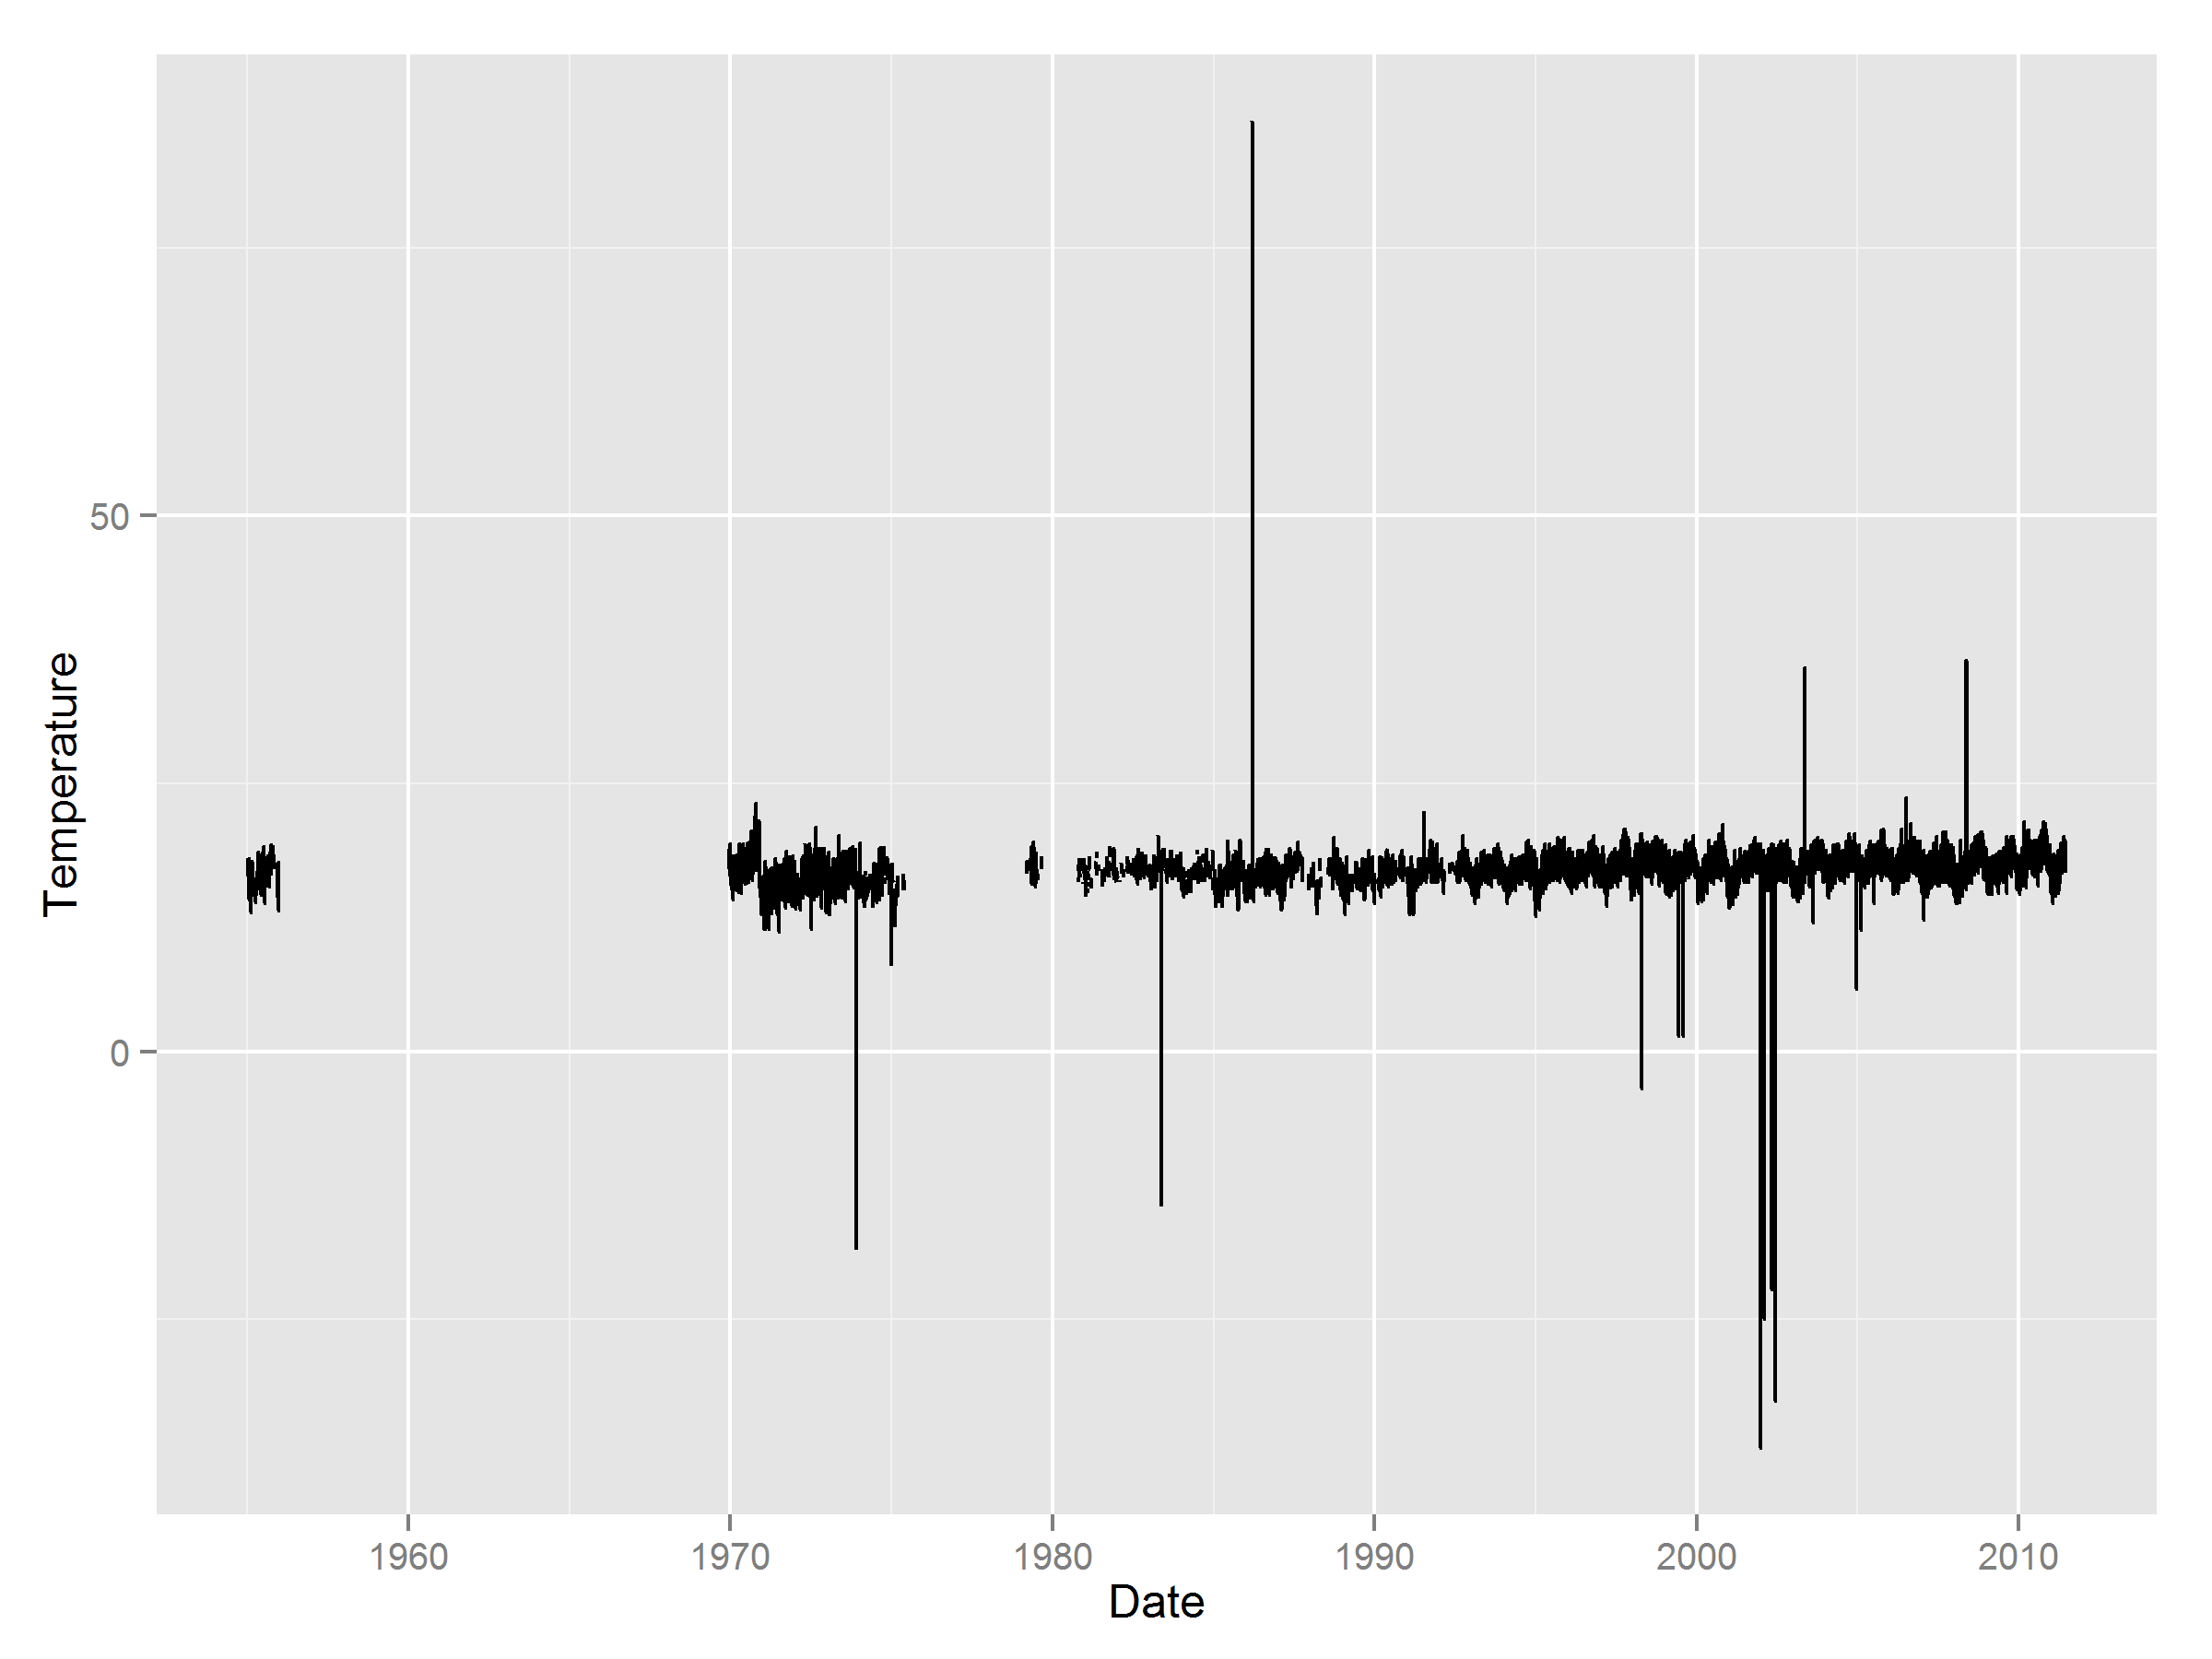
\includegraphics[width=.5\textwidth]{Temperature_data_from_mandy_outliers} &
		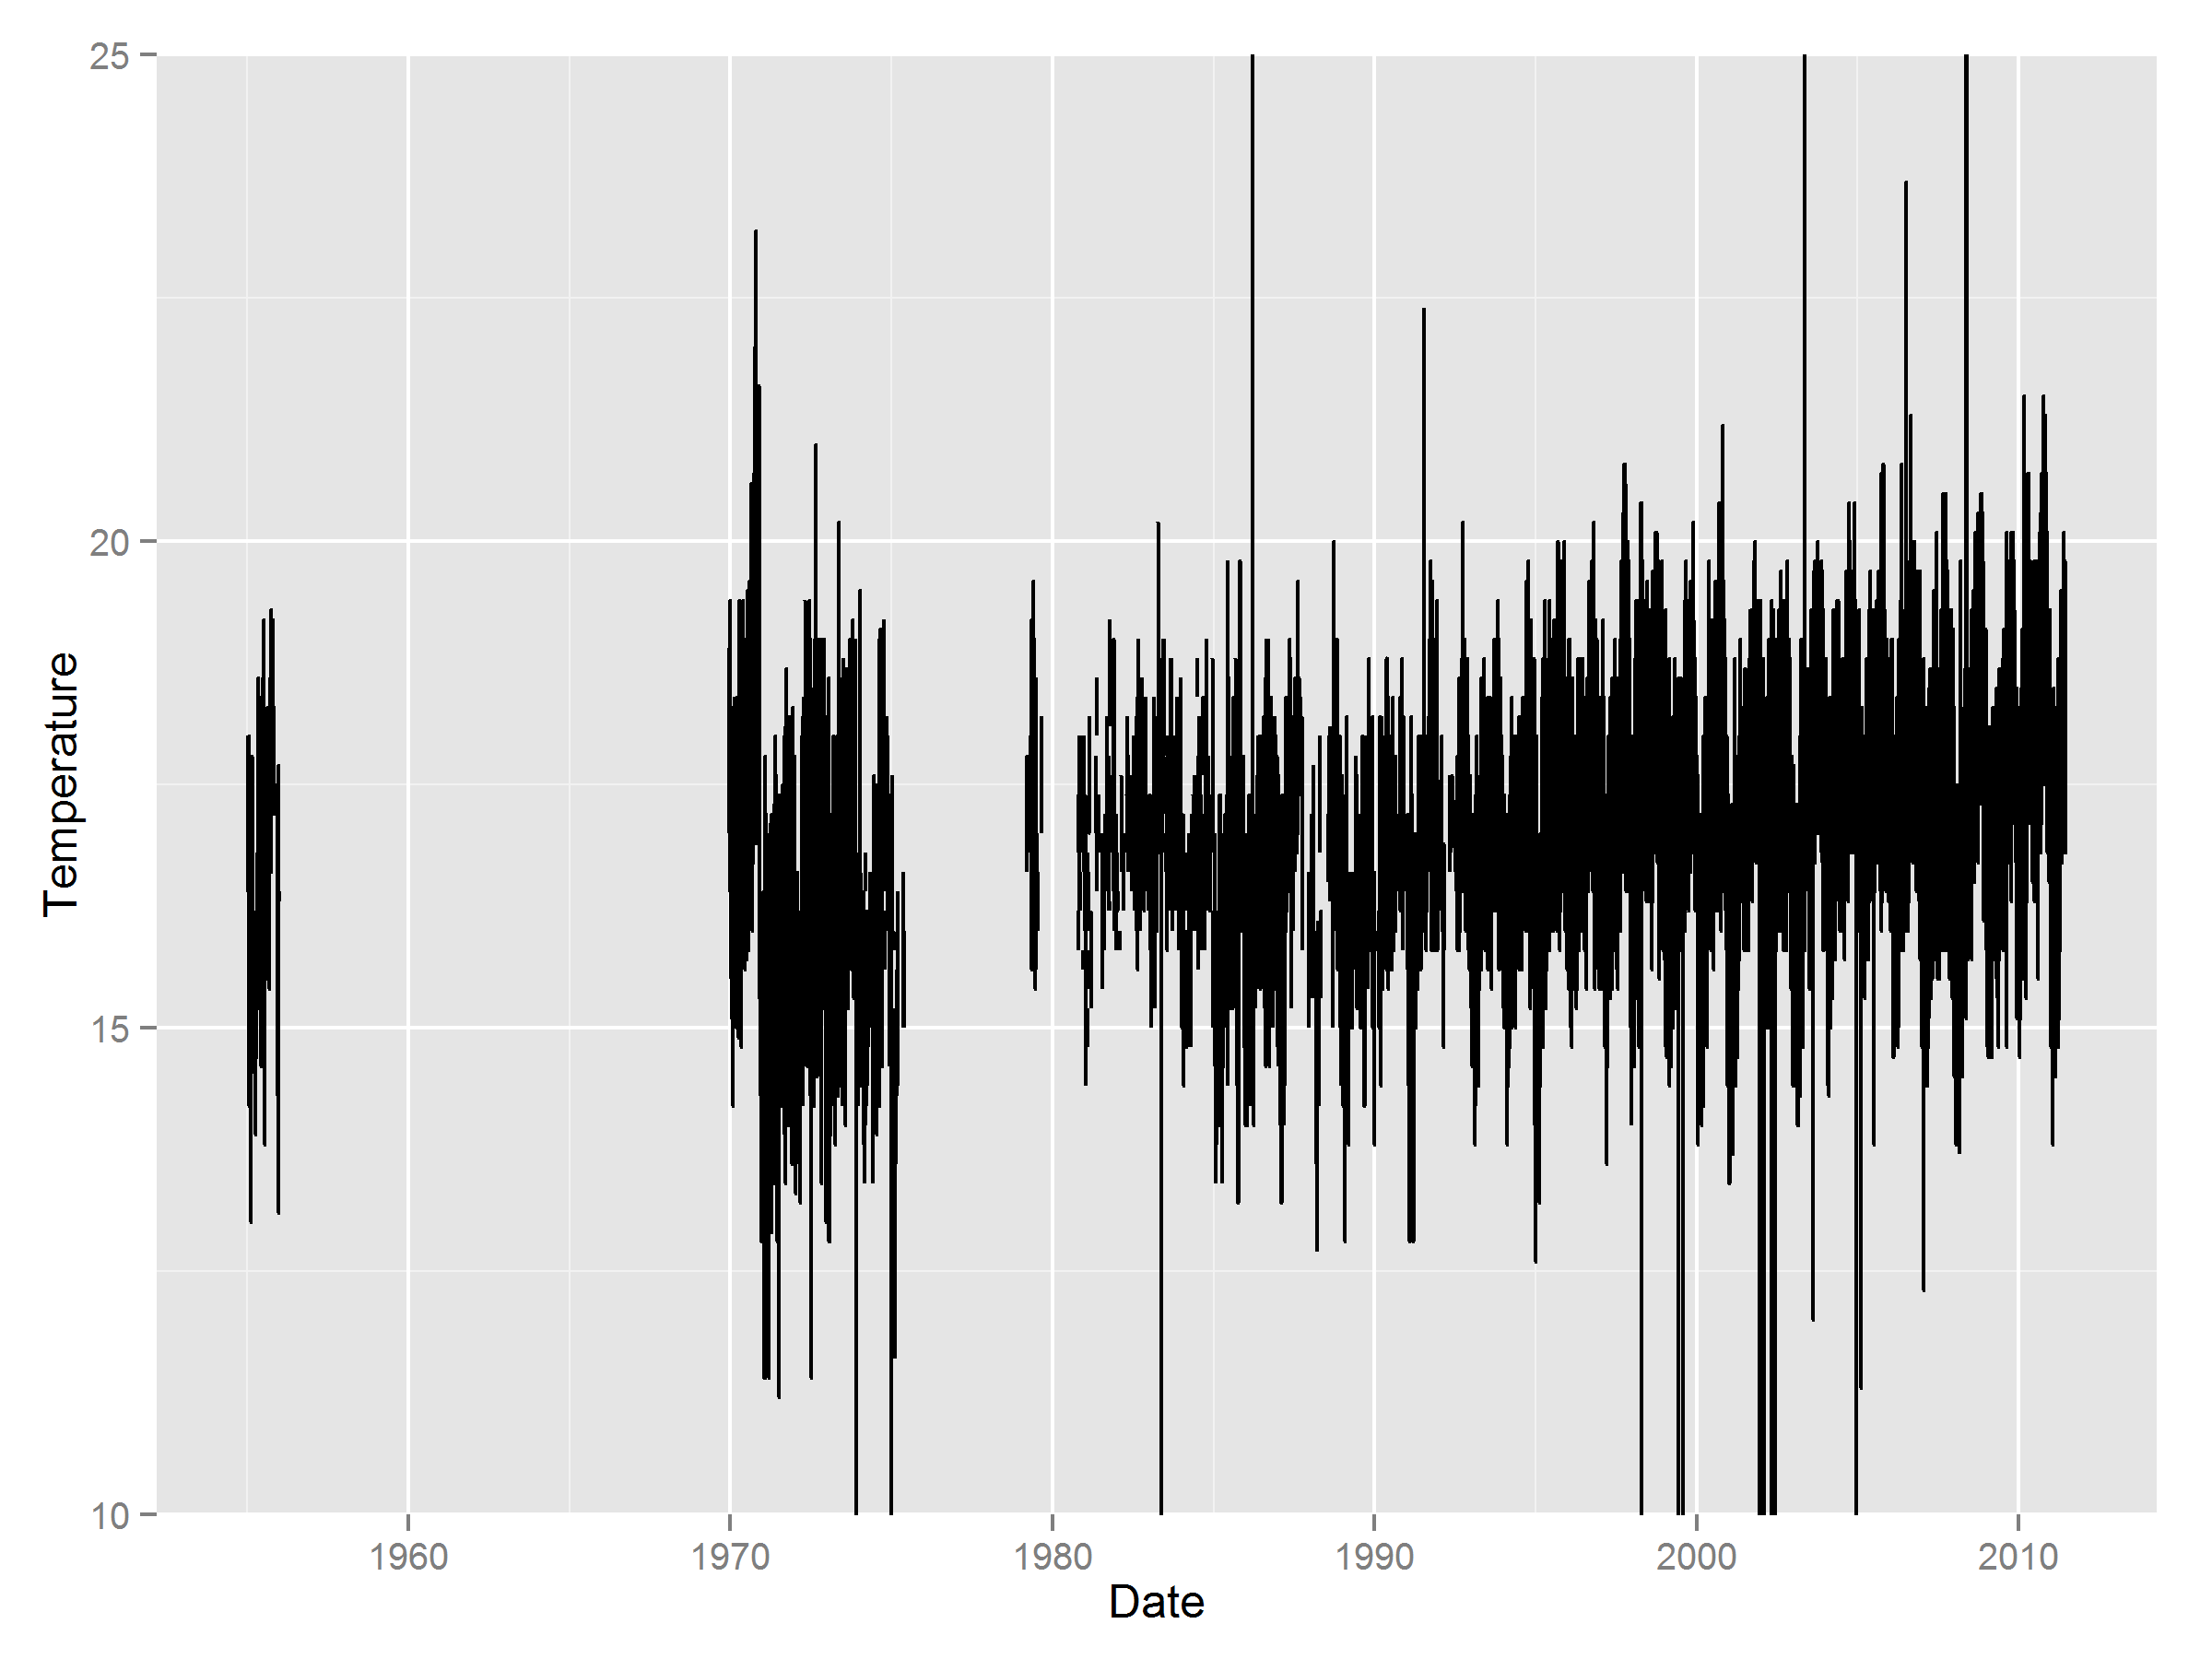
\includegraphics[width=.5\textwidth]{Temperature_data_from_mandy_changepoints}
	\end{tabular}
	\caption{Temperature for Station \textbf{???} plotted over time.  The second image is the same as the first but with a smaller $y$-axis window so as to show more detail.}
	\label{fig:BasicTS}
\end{figure}

\begin{figure}[h!]
	\centering
	\includegraphics[width=\textwidth]{final_paper_efficiency_plot_35121_10_N_Y}
	\caption{Boxplot of efficiency scores for the various homogenization algorithms.}
	\label{fig:hom_Efficiency}
\end{figure}

\begin{figure}[h!]
	\centering
	\includegraphics[width=\textwidth]{final_paper_trend_penalty_35121_10_N_Y}
	\caption{Estimates of trend from homogenized data.  ``Raw'' method indicates no homogenization has been performed, and the red dashed line is the true/simulated trend.}
	\label{fig:hom_Trend}
\end{figure}

\begin{figure}[h!]
	\centering
	\begin{tabular}{cc}
		\includegraphics[width=.5\textwidth]{FINAL_TPR_Interaction_Plot_Order_OutlierPct} &
		\includegraphics[width=.5\textwidth]{FINAL_TPR_Interaction_Plot_Order_SimBrCnt}
	\end{tabular}
	\caption{Mean true positive rate for the various quality control methods.  The bands represent the 2.5\% and 97.5\% quantiles for all simulations.}
	\label{fig:TPR}
\end{figure}

\begin{figure}[h!]
	\centering
	\begin{tabular}{cc}
		\includegraphics[width=.5\textwidth]{FINAL_Efficiency_Interaction_Plot_SimBreaks_OutlierPct} &
		\includegraphics[width=.5\textwidth]{FINAL_Efficiency_QC_Order}
	\end{tabular}
	\caption{Mean efficiency for the various quality control methods.  The bands represent the 2.5\% and 97.5\% quantiles for all simulations.}
	\label{fig:Efficiency}
\end{figure}
\end{document}